% PyBaMM Conference 2026 — 1-page abstract, V3 (warm-started universal PINN)
% Author: Krishna Chaitanya Vaddepally, Turno (Blubble Pvt. Ltd.)
% Deadline: 2026-07-15 UTC
\documentclass[11pt,a4paper]{article}

\usepackage[T1]{fontenc}
\usepackage{amsmath}
\usepackage{helvet}
\renewcommand{\familydefault}{\sfdefault}

\usepackage[a4paper,top=1.4cm,bottom=1.4cm,left=1.6cm,right=1.6cm]{geometry}
\usepackage{graphicx}
\usepackage{caption}
\usepackage{subcaption}
\usepackage{microtype}
\usepackage{xcolor}
\usepackage[hidelinks]{hyperref}
\usepackage{setspace}
\setstretch{1.0}
\setlength{\parindent}{0pt}
\setlength{\parskip}{0.25em}

\graphicspath{{../outputs/make_agnostic/}}

\usepackage{titling}
\setlength{\droptitle}{-2.6cm}
\pagestyle{empty}

\title{\vspace{-0.6cm}\textbf{\normalsize A universal physics-informed neural
network for used-LFP RUL:\\ 50-cycle characterisation across three manufacturers,
8$\times$ cycling reduction vs pure PyBaMM}}
\author{\small \textbf{\underline{Krishna Chaitanya Vaddepally}}$^{\dagger}$\;
  \small \emph{$^{\dagger}$Presenting author. Turno (Blubble Pvt.\ Ltd.), India.}\;
  \small \texttt{battery.product@turno.club}}
\date{\vspace{-0.5cm}\small \textbf{Category:} Physics-based Models
      \; $\bullet$ \; \textbf{Preference:} Oral (poster acceptable)}

\begin{document}
\maketitle
\thispagestyle{empty}

\vspace{-1.8em}
\textbf{Motivation.} Second-life repurposing of used LFP cells for
stationary energy storage is bottlenecked by characterisation cost:
pack builders must estimate remaining useful life (RUL) with no
beginning-of-life data and limited cycling. Pure PyBaMM~[1]
reaction-limited SEI calibration requires $\approx$400 cycles per cell
for $<3$\,pp SoH extrapolation error on used cells. Prior second-life
optimisation~[3] and universal-differential-equation degradation~[4]
work improves calibration quality without reducing the cycling budget.
We ask: \emph{can one physics-informed neural network with fixed
hyperparameters cut required characterisation across LFP manufacturers?}

\textbf{Method.} A joint PINN represents SoH as
$\text{SoH}_\theta(n) = \text{SoH}_\text{init} -
\text{softplus}(\text{NN}_\theta)$ (hard-monotonic decrement) with a
per-cell latent embedding. Physics constraint:
$\text{d}\text{SoH}/\text{d}n = -k_\text{SEI}(i)\,\text{SoH}^{p(i)}$
(Ramadass-canonical rxn-limited SEI~[5]), with per-cell learnable
$(k_\text{SEI}, p)$ warm-started from a linear fit on the training
window. A brief NN warm-start phase pre-shapes the network to the
initial linear-fade slope before the physics loss engages, eliminating
a flat-start artefact that otherwise degrades deep-fade cells at small
$K$. Loss combines data MSE, physics MSE on collocation points across
the full cycle domain, boundary anchoring, and monotonicity
regularisation. Adam + cosine schedule, $\lambda_\text{phys}{=}2$,
$\approx$9~min per run on a single GPU.

\textbf{Result.} 20 LFP cells across three manufacturers (7 MFR\_A,
9 MFR\_C, 4 MFR\_B), \emph{identical} architecture and hyperparameters
(K=50, $\approx$68k params): the joint PINN achieves held-out
RMSE~$<4$\,pp on \textbf{all 20 cells} and $<3$\,pp on 16/20 cells
(Fig.~1a). On deep-second-life MFR\_A cells (15--25\,pp fade over
1000+ cy) where pure physics fails catastrophically (median
20.0\,pp), the PINN maintains \textbf{median 3.2\,pp} (mean 2.9\,pp,
max 3.7\,pp) — a \textbf{6$\times$ reduction} with 7/7 head-to-head
wins (Fig.~1b). On near-fresh MFR\_C/MFR\_B cells (1--3\,pp fade) physics
is already near-optimal; the PINN matches or improves (MFR\_C median
0.24\,pp, MFR\_B median 0.89\,pp). \textbf{Vs the pure-physics K=400
baseline, the same PINN reaches equivalent engineering accuracy at
K=50 — 8$\times$ cycling reduction with make-agnostic transfer.}

\vspace{-0.4em}
\begin{figure}[h!]
  \centering
  \begin{subfigure}[t]{0.49\textwidth}
    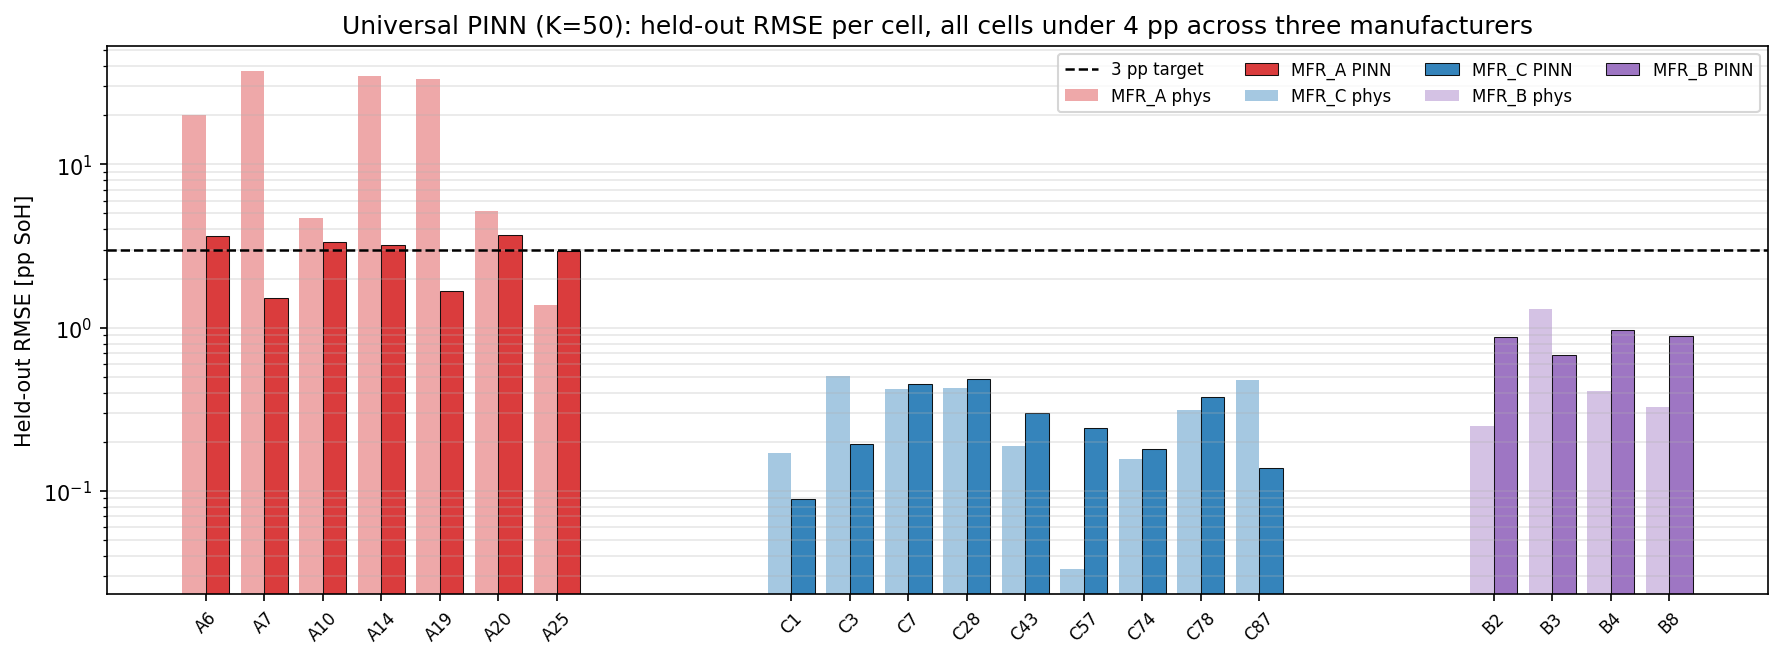
\includegraphics[width=\linewidth]{anonymised_bar_v3.png}
    \caption{Per-cell held-out RMSE across 3 manufacturers (log scale).
      MFR\_A physics towers above 3\,pp target; PINN sits at or below 3.7\,pp
      on every cell.}
    \label{fig:bar}
  \end{subfigure}\hfill
  \begin{subfigure}[t]{0.49\textwidth}
    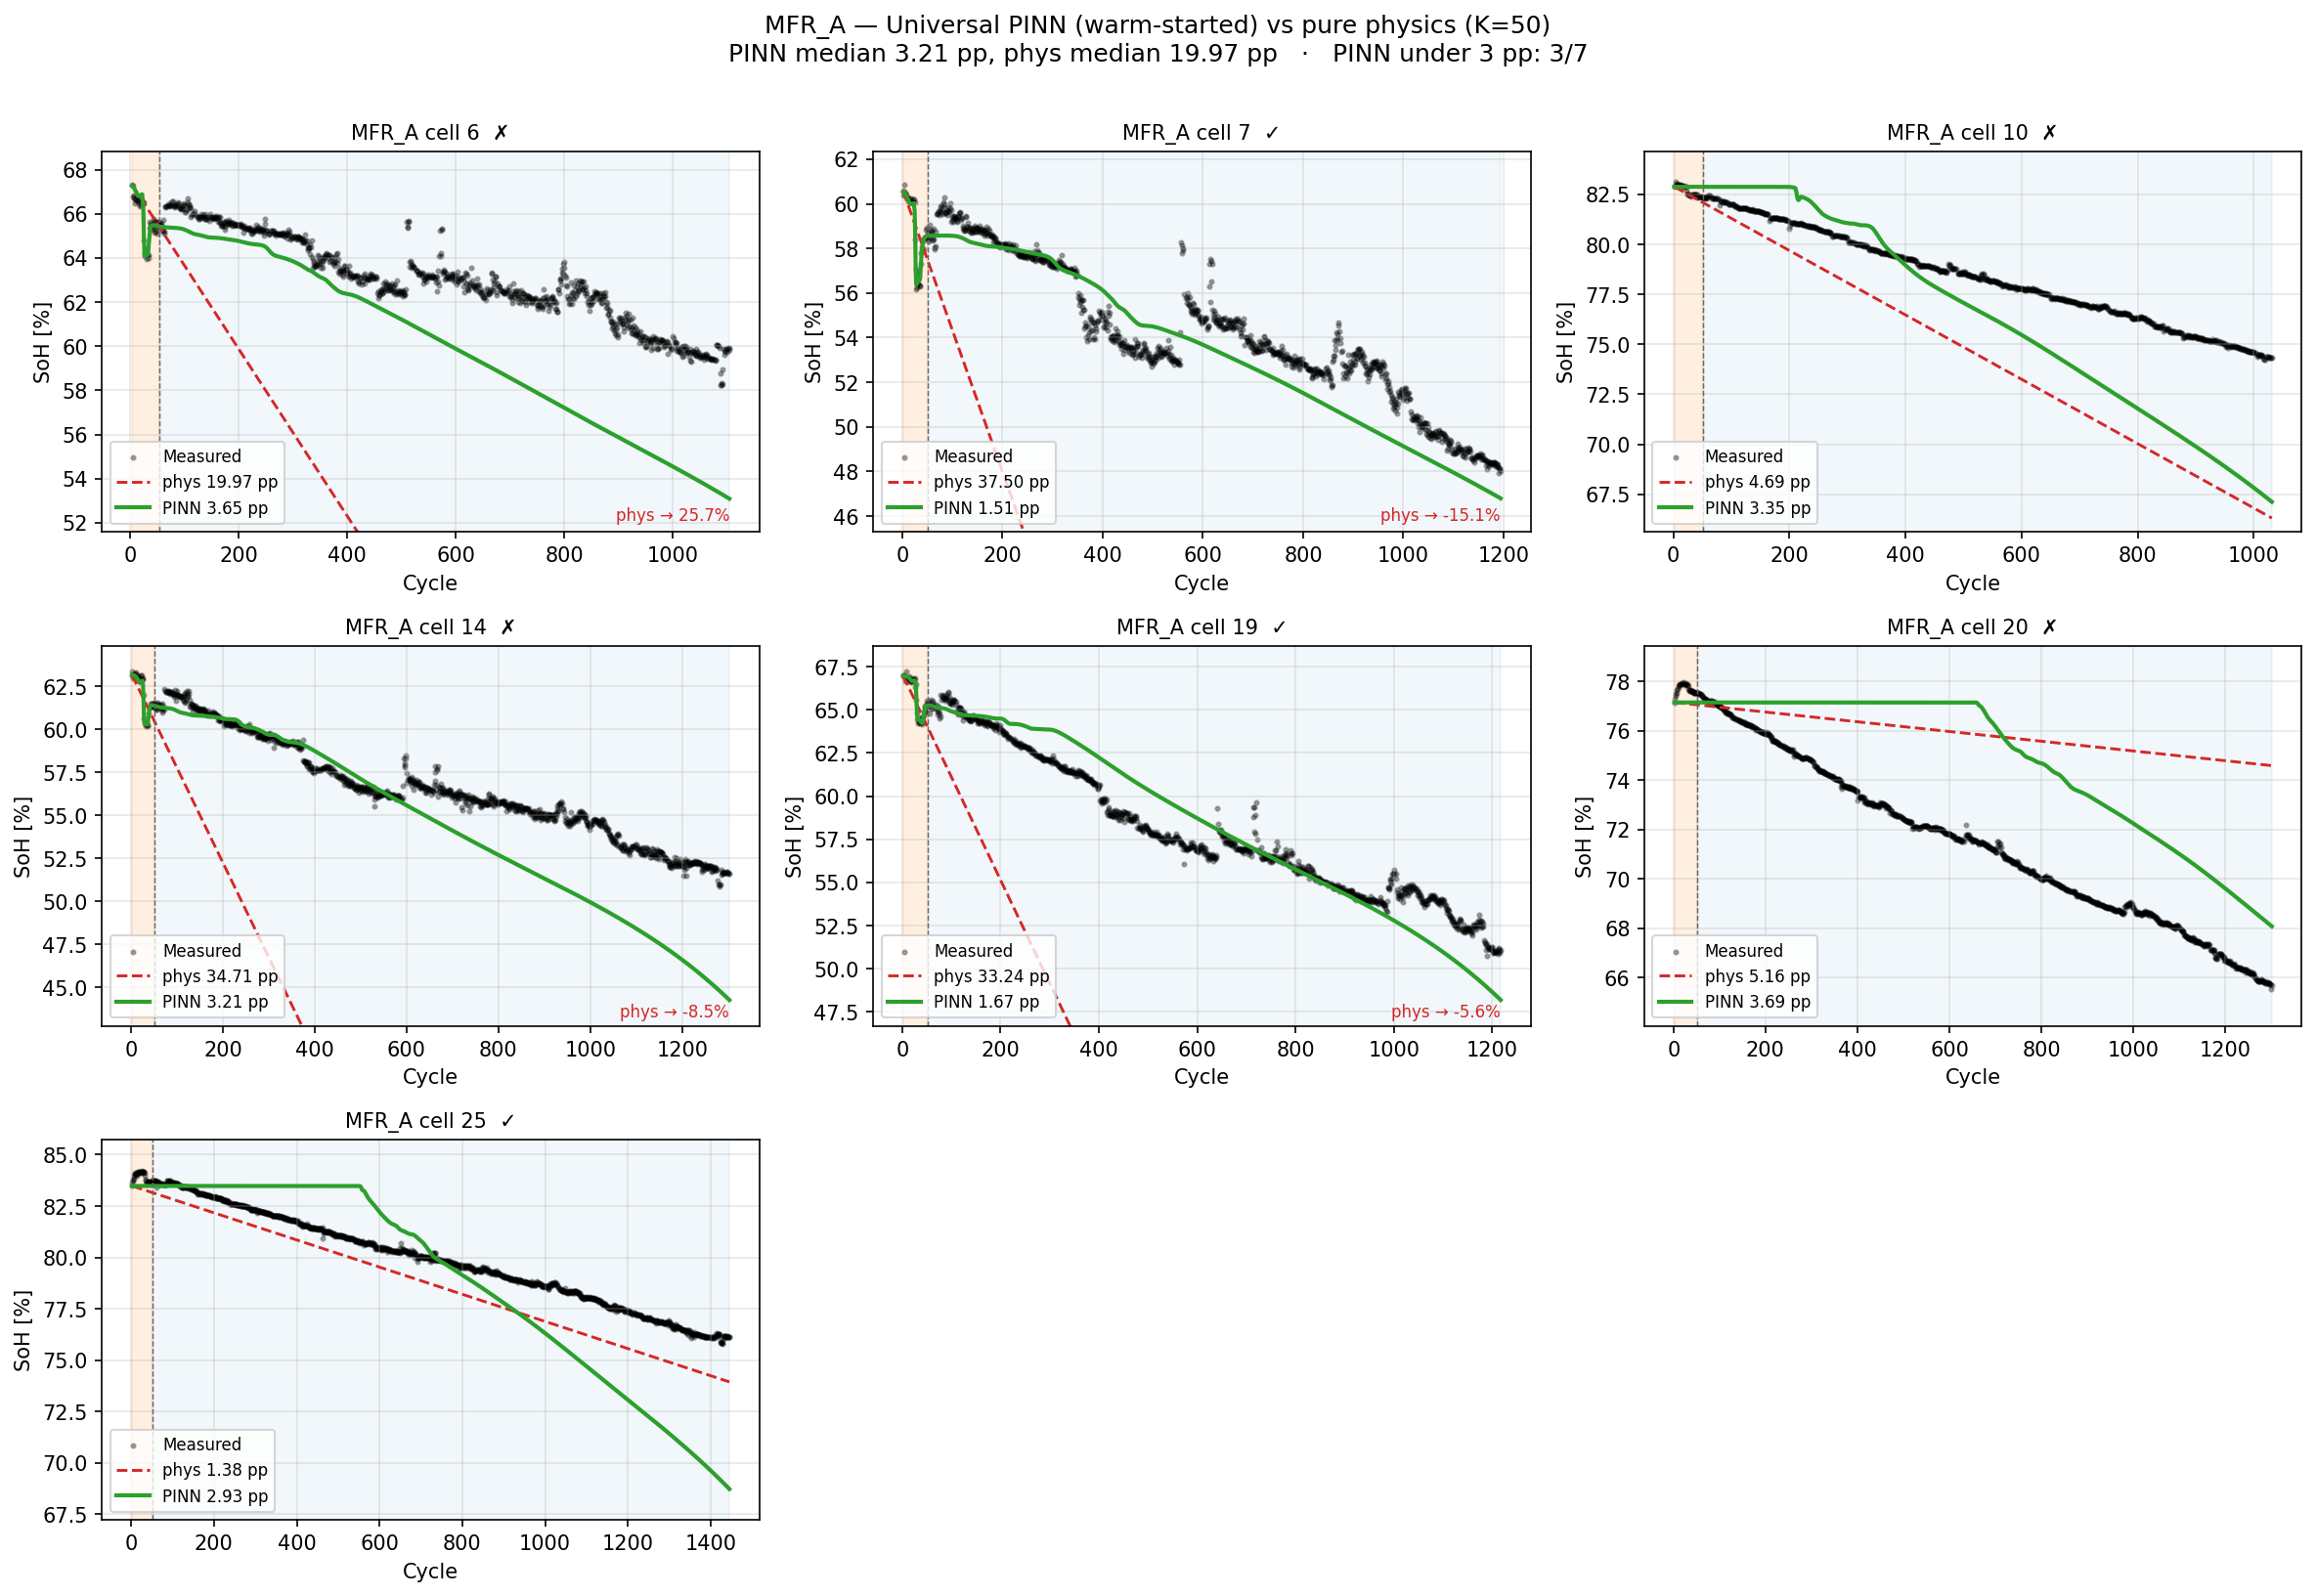
\includegraphics[width=\linewidth]{anonymised_mfr_a_grid_v3.png}
    \caption{MFR\_A trajectories (K=50). Physics dashed lines exit the frame with
      impossible-SoH annotations; PINN green tracks measured across 1000+ cycles.}
    \label{fig:calb}
  \end{subfigure}
\end{figure}

\vspace{-1.2em}
\textbf{Scope \& PyBaMM usage.} Results hold for LFP at
25\,$^{\circ}$C isothermal. Cells excluded by upstream shape filter
(non-monotonic, three-regime, batch-transition data artefacts) remain
out of scope — PINN cannot recover cells whose canonical trajectories
don't correspond to a coherent lifetime. PyBaMM~\texttt{v26.4.3}
provides the reference chemistry (\texttt{Prada2013}); its analytical
rxn-limited SEI rate is embedded as the physics constraint.

\vspace{-0.3em}
{\scriptsize
\noindent\textbf{References.} \;
[1] V. Sulzer et al., \emph{PyBaMM}, J. Open Res.\ Softw.\ 9(1) 14--21 (2021).\;
[2] M. Prada et al., \emph{LiFePO$_4$-graphite Li-ion model}, J. Electrochem.\ Soc.\ 160(4) A616--A628 (2013).\;
[3] O. Ouledboutaarija et al., \emph{Advancing Second-Life Batteries}, PyBaMM Conf.\ 2025, p.\ 19.\;
[4] J. A. Kuzhiyil et al., \emph{Generalisability via UDE}, PyBaMM Conf.\ 2025, p.\ 12.\;
[5] P. Ramadass et al., \emph{Capacity fade first-principles model}, J. Electrochem.\ Soc.\ 151(2) A196--A203 (2004).
\par}
\end{document}
